\chapter{Basic 2D Network on Chip model}
\label{Chapter.five}

In this chapter, we present a basic 2D Network on Chip (NoC) agent based model using the classes in GeoMason~\cite{GEOMASON2011,GEOMASON} Library. The 2D NoC model consists of a self routing agent moving along the 2D mesh network and following XY-routing algorithm. The architecture of this model is further explained in the following section. 

\section{Architecture}

The 2D NoC agent based model is designed using GeoMason classes such as GeomVectorField~\cite{GEOMV} and GeomPlanarGraph~\cite{GEOMPG}. This model consists of an Environment, a NodeElement and a Packet agent which are described below. 


\vspace{0.3cm}
\noindent\textbf{Environment}
\vspace{4mm}

\noindent The Environment chosen for this 2D NoC agent based model is 4x4 2D mesh network. This environment is created by using a LineString class and a node at intersection of the each LineString. Environment consists of NodeElement and Packets.

\vspace{0.5cm}
\noindent\textbf{NodeElement}
\vspace{5mm}

\noindent The NodeElement is the place where the Packets are created and scheduled. A NodeElement is created and scheduled from a ``Noc.java'' class.  
 
\vspace{0.3cm}
\noindent\textbf{Packet}
\vspace{5mm}

\noindent A Packet is a self routing agent. Packets are created at the NodeElement class. A Packet follows the XY-routing algorithm to travel from a source to a destination. XY- routing algorithm used in the model is explained below:

\vspace{10 mm} 
\algdef{SE}[IF]{NoThenIf}{EndIf}[1]{\algorithmicif\ #1}{\algorithmicend\ \algorithmicif}
\begin{algorithm}[H]
\small % remove to adjust the position and size%
\caption{XY Routing Algorithm}
\label{alg5.1}
\begin{boxedminipage}{150mm}
\vspace{5mm}
\begin{algorithmic}[1]
\NoThenIf{$(Dx>Cx)$} 
\State Move the Packet to East;
\ElsIf{$(Dx<Cx)$} 
\State Move the Packet West;
\ElsIf{$(Dx=Cx)$}
\NoThenIf{$(Dy>Cy)$} 
\State Move the Packet North;
\ElsIf{$(Dy<Cy)$}  
\State Move the Packet South;
\Else  
\State Packet reached its destination address (Dx, Dy);
\EndIf
\EndIf
\end{algorithmic}
\vspace{5mm}
\end{boxedminipage}
\end{algorithm}
\vspace{10 mm}


Algorithm~\ref{alg5.1} is as follows: Current address of a Packet is $(Cx, Cy)$ and destination address is $(Dx, Dy)$. Firstly, the X-coordinate of the current address $(Cx)$ is compared to the X-coordinate of the destination address $(Dx)$. Packet moves towards East when $Dx>Cx$, towards West when $Dx<Cx$, and if $Dx=Cx$ it has already aligned in the destination address's X-coordinate $(Dx)$. Finally, $Cy$ is compared with $Dy$. When $Dy>Cy$ the Packet moves towards North, when $Dy<Cy$ it moves towards South and when $Dy=Cy$ the packet stops moving further as it has reached its final destination. When all the packets have reached their destinations the schedule ends. 


\begin{figure}[H]
\vspace{10 mm}
\centering
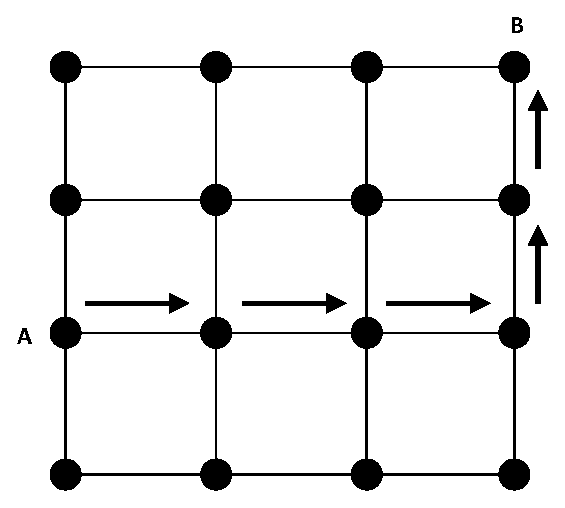
\includegraphics[width=.5\linewidth]{2DmeshXY.eps}
\caption{2D Mesh Network with XY-routing}
\label{fig:5.1}
\vspace{10 mm}
\end{figure} 

In Fig.\ref{fig:5.1}, we can see a 2D mesh Network with ``A'' as a current address of the Packet and ``B'' as a destination address. According to the XY-routing algorithm, A Packet from ``A'' will traverse through the marked route in Fig.\ref{fig:5.1} to reach ``B''. Packet travels in X-direction (horizontally) until it reaches the correct column and then it travels in Y-direction (vertically) till it reach the destination address.

\subsection{Running the Model}

When the model is scheduled, the windows looks like as shown in Fig.\ref{fig:5.2}. In the right window, we can see an ``html'' page displaying the description of model. Window on the left is the actual schedule, where agents traverse in the environment. The window on the right side has three buttons: play, pause and stop. With the help of these buttons, we can play, pause and stop the schedule. When we click on play button, the schedule starts. When schedule begins, packets start moving from their respective nodes. Green color spheres represent nodes in the network. White color spheres are Packets. NodeElements can be seen as red color spheres. When all the packets reach their destination the schedule stops.
 
\begin{figure}[H]
\vspace{15 mm}
\flushleft
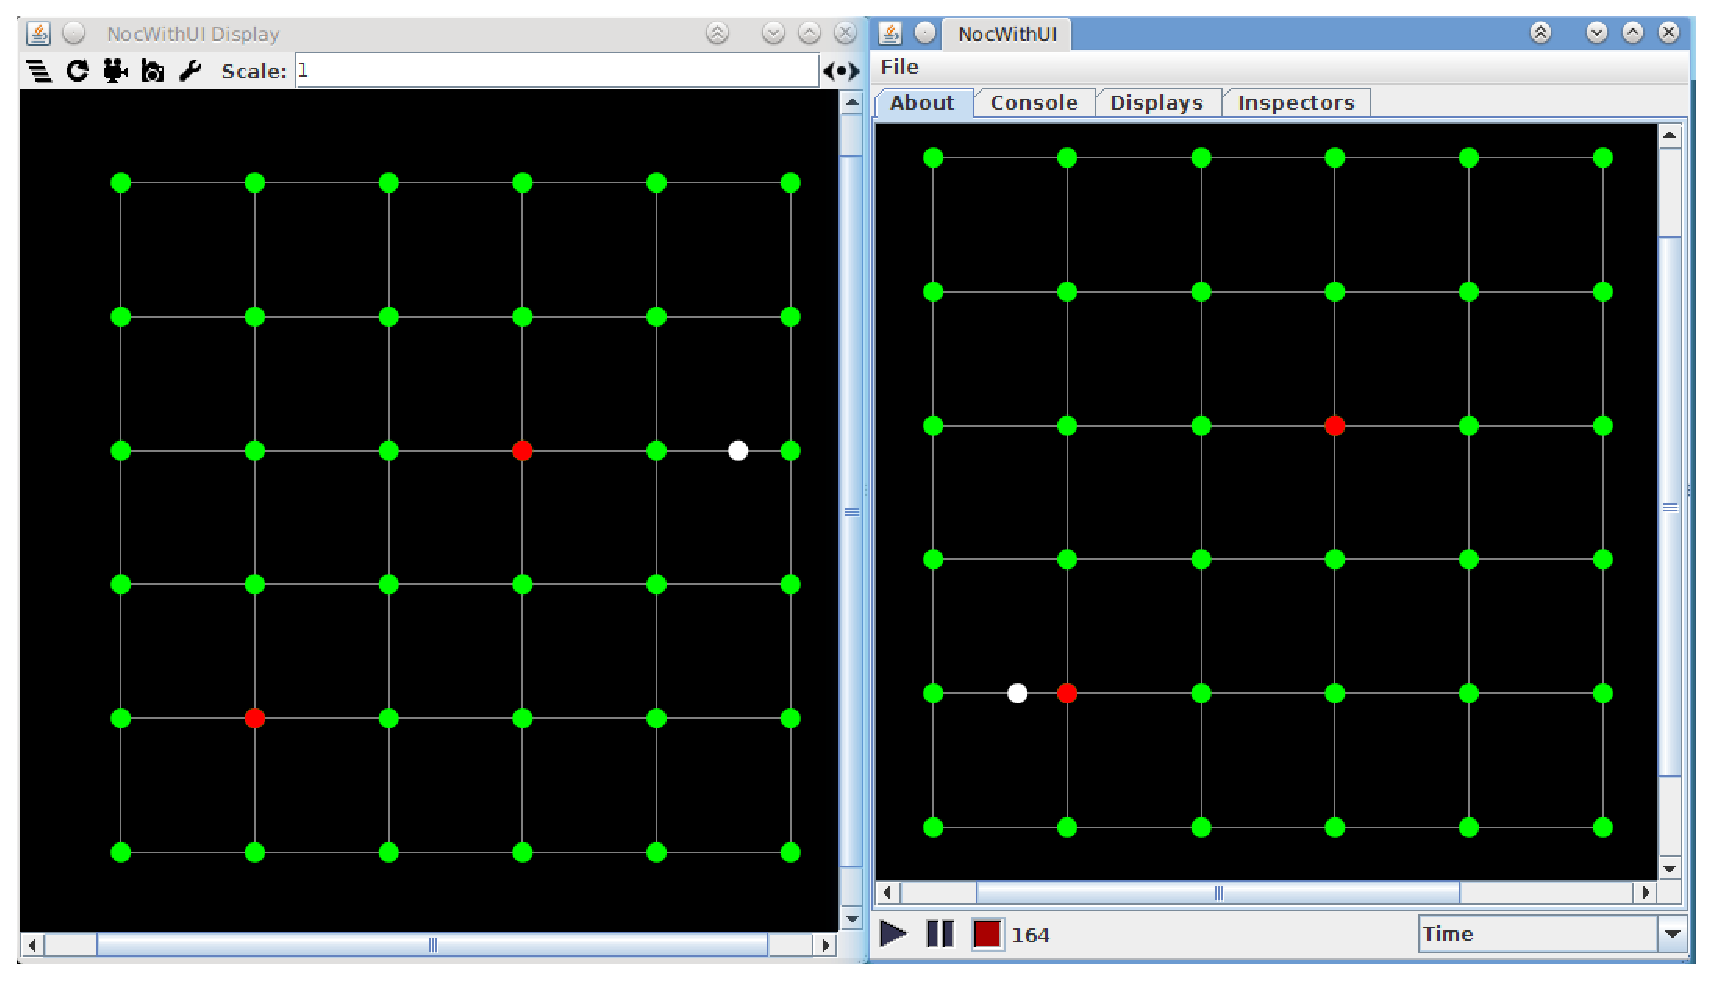
\includegraphics[height=5.1in, width=5.9in]{noc2d.eps}
%\includegraphics[width=.54\linewidth]{noc2D.eps}
\caption{Scheduling 2D NoC}
\label{fig:5.2}
\vspace{10 mm}
\end{figure} 

\section{Procedure}

Designing a 2D NoC agent based model using GeoMason classes involves the following steps.

\begin{enumerate}
 \item Create a package named $noc2d$ in app folder of the tool. Create all the classes in $noc2d$ package.
 \item Create a class ~\texttt{Noc2D}. In ~\texttt{Noc2D} the environment is created using Java classes.
 \item Create a ~\texttt{NodeElement} class for creating Packets.
 \item Design a self routing agent which moves along the 2D network and follows XY-Routing algorithm. Self routing agent gets the location information from the ~\texttt{Noc2D} class in order to navigate between the nodes. This information can be retrieved by creating and using the objects of the ~\texttt{Noc2D} class.
 \item Create a class ~\texttt{Noc2DWithUI} which extend the ~\texttt{GUIState} class.~\texttt{GUIState} class enables visualization to MASON models.
 \item When we run ~\texttt{Noc2DWithUI}, all the other classes starts their schedule and runs until $``exit''$ command is encountered.
 \item Run model using command $``java~sim.app.noc2d.Noc2DWithUI''$.
\end{enumerate}
\vspace{5mm}

After modeling a 2D NoC, the next step is to create a 3D NoC agent based model. We use MASON 3D classes in this model because the support provided by GeoMason classes is not sufficient to create our 3D NoC model. We introduce our 3D 4x4 mesh NoC agent based model in the next chapter.
 



  

 


